\documentclass[tikz]{standalone}
\usepackage[english]{babel}
\usepackage{amsmath}
\usepackage{amssymb}
\usepackage[T1]{fontenc}
\usepackage[default]{droidsans}
\usepackage[LGRgreek]{mathastext}
\usetikzlibrary{arrows.meta,calc,decorations.markings,decorations.pathmorphing,positioning}
\begin{document}
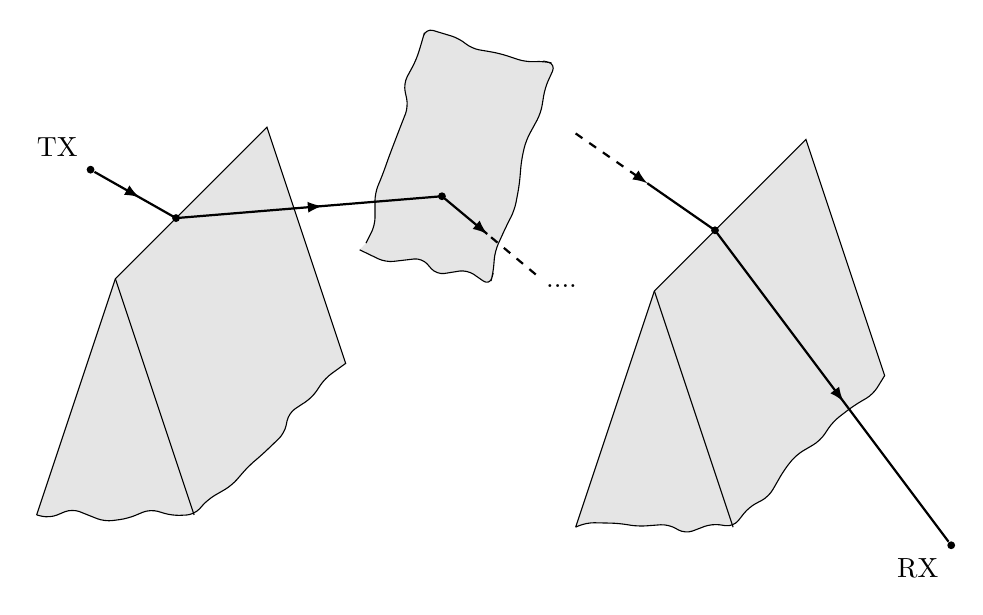
\begin{tikzpicture}[decoration={random steps,segment length=3mm}]
  \pgfmathsetseed{42}
  \node[circle,fill,inner sep=1pt,label=above left:{TX}] (tx) at (0.3,4,-1) {};
  \node[circle,fill,inner sep=1pt,label=below left:{RX}] (rx) at (12,0,1) {};

  \begin{scope}
    \coordinate (e11) at (0,0,0);
    \coordinate (e12) at (2,0,0);
    \coordinate (e13) at (1,3,0);
    \coordinate (e14) at (2,0,-5);
    \coordinate (e15) at (1,3,-5);
    \coordinate (o1) at (1,3,-1);
    \coordinate (x1) at (1,3,-2);
    \coordinate (e1) at (1,3,-6);

    \filldraw[fill=gray!20] (e11) -- (e13) -- (e15) -- (e14) decorate[rounded corners=1mm] { -- (e12)} decorate[rounded corners=1mm] { -- (e11) };
    \draw (e12) -- (e13);

    \node[circle,fill,inner sep=1pt] at (x1) {};
  \end{scope}

  \begin{scope}[shift={(3,2.2,-3)}]
    \coordinate (p21) at (0,0,0);
    \coordinate (p22) at (0,2,-2);
    \coordinate (p23) at (2,2,-1);
    \coordinate (p24) at (2,0,1);
    \coordinate (o2) at (1,1,-.5);
    \coordinate (x2) at (0.8,0.5,-.5);
    \coordinate (u2) at (1,2.5,-1.5);
    \coordinate (v2) at (-.5,1.25,-.5);
    \coordinate (x3) at (2.5,0.0,+0.8);
    \node[below right] at (x3) {....};

    \filldraw[fill=gray!20,decorate,rounded corners=1mm] (p21) -- (p22) -- (p23) -- (p24) -- cycle;

    \node[circle,fill,inner sep=1pt] at (x2) {};
  \end{scope}

  \begin{scope}[shift={(8,1,+3)}]
    \coordinate (en1) at (0,0,0);
    \coordinate (en2) at (2,0,0);
    \coordinate (en3) at (1,3,0);
    \coordinate (en4) at (2,0,-5);
    \coordinate (en5) at (1,3,-5);
    \coordinate (on) at (1,3,-1);
    \coordinate (xn) at (1,3,-2);
    \coordinate (xnm1) at (0,5,0);
    \coordinate (en) at (1,3,-6);

    \filldraw[fill=gray!20] (en1) -- (en3) -- (en5) -- (en4) decorate[rounded corners=1mm] { -- (en2)} decorate[rounded corners=1mm] { -- (en1) };
    \draw (en2) -- (en3);

    \node[circle,fill,inner sep=1pt] at (xn) {};
  \end{scope}

  \begin{scope}[dashed,decoration={
        markings,
      mark=at position 1 with {\arrow{latex}}}
    ]
    \path (x2) -- (x3) node[midway,inner sep=0pt] (midx2x3) {};
    \draw[thick,solid,postaction={decorate}] (x2) -- (midx2x3);
    \draw[thick,dashed] (midx2x3) -- (x3);
  \end{scope}

  \begin{scope}[decoration={
        markings,
      mark=at position 0 with {\arrow{latex}}}
    ]
    \path (xnm1) -- (xn) node[midway,inner sep=0pt] (midxnm1xn) {};
    \draw[thick,dashed] (xnm1) -- (midxnm1xn);
    \draw[thick,solid,postaction={decorate}] (midxnm1xn) -- (xn);
  \end{scope}

  \begin{scope}[thick,decoration={
        markings,
      mark=at position 0.55 with {\arrow{latex}}}
    ]
    \draw[postaction={decorate}] (tx) -- (x1);
    \draw[postaction={decorate}] (x1) -- (x2);
    \draw[postaction={decorate}] (xn) -- (rx);
  \end{scope}

\end{tikzpicture}
\end{document}
